\documentclass[../main.tex]{subfiles}
\begin{document}

\chapter{Überblick}
\label{overview}
\pagenumbering{arabic}
  Die Virtualisierung entwickelte sich in den letzten Jahren zu einem allgegenwärtigen Thema in der Informatik. Mehrere Virtualisierungstypen entstanden, als von akademischen und industriellen Forschungsgruppen vielseitige Einsatzmöglichkeiten der Virtualisierung aufgedeckt wurden.

  Allgemein versteht man unter ihr die Nachahmung und Abstraktion von physischen Ressourcen, z.B. der \acrshort{CPU} oder des Speichers, die in einem virtuellen Kontext von Programmen genutzt wird.

  Die Vorteile von Virtualisierung umfassen Hardwareunabhängigkeit, Verfügbarkeit, Isolierung und Sicherheit, welche die Erfolgsgrundlage von heutigen \gls{Cloud}-Infrastrukturen in Rechenzentren bilden \cite[S.1]{containerVirtPerformance}.
  %V.a. in Rechenzentren bieten sich Virtualisierungslösungen an, um die Serverressourcen effizienter zu nutzen \cite[S.1]{dockerSec1}.
  Letztendlich haben es Virtualisierungslösungen ermöglicht, Dienste von Clouds, wie z.B. den \emph{Amazon Web Services}\cite{amazonWebServices}, auf Basis eines Subskriptionsmodells nutzen zu können \cite[S.1]{dockerSec1}.

  Heutzutage existieren mehrere serverseitige Virtualisierungstechniken, wovon die hypervisorgestützten Methoden mit den etablierten Vertretern \emph{Xen} \cite{xen}, \emph{KVM} \cite{kvm}, \emph{VMware ESXi} \cite{vmwareESXi} und \emph{Hyper-V} \cite{hyperv} die meistverbreitesten sind \cite[S.2]{containerVirtPerformance}. Die alternative containerbasierte Virtualisierung, auch Virtualisierung auf Betriebssystemebene genannt, wurde in den letzten Jahren durch ihre leichtgewichtige Natur zunehmend beliebt und erlebte mit dem Erfolg von Docker, seit dessen Release im März 2013, einen medienwirksamen Aufschwung \cite{githubDockerChangelog}. Wie die \emph{Google Trends} in \fig \ref{fig:overview_googleTrends} zeigen, stieg das Interesse an Docker seit dessen Release kontinuierlich an. Das Interesse an der Containertechnologie \emph{LXC}, aus der Docker entstand, bleibt weit hinter der von Docker zurück. Das Suchwort \glqq{}Virtualization\grqq{} erlebte im Jahr 2010 seinen Höhepunkt und hat seitdem an Popularität verloren \cite{googleTrends}. Obwohl Docker eine Art von  Virtualisierungstechnologie ist, wird der Begriff der Virtualisierung meist mit tradiotioneller hypervisorbasierter Virtualisierung verbunden. Der Virtualisierungsaspekt von Docker wird dagegen meist mit Containern beschrieben.

  \begin{figure}[h]
      \centering
      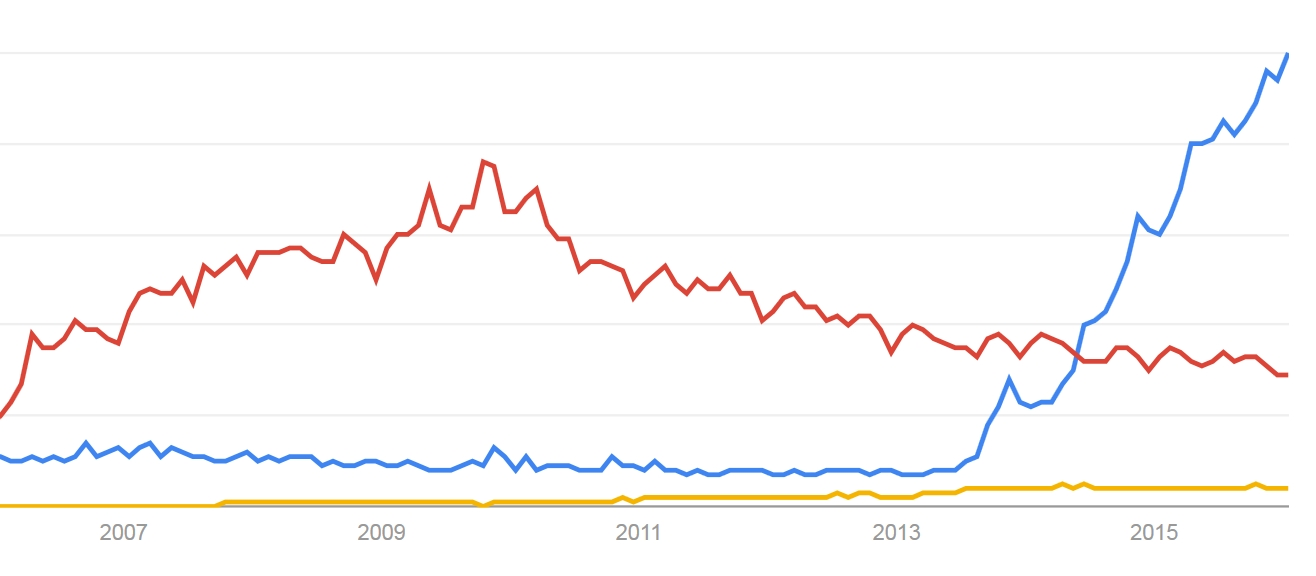
\includegraphics[width=1.0\textwidth]{./images/googletrend_dockerVirtualizationLXC.jpg}
      \caption{Google Trends der Suchbegriffe \glqq{}Virtualization\grqq{} (rot), \glqq{}Docker\grqq{} (blau) und \glqq{}LXC\grqq{} (gelb) von Januar 2006 bis Januar 2016\cite{googleTrends}.}
      \label{fig:overview_googleTrends}
  \end{figure}

  Obwohl das Konzept von Containern bereits im Jahr 2000 als \emph{Jails} in dem Betriebssystem \emph{FreeBSD} und seit 2004 als \emph{Zones} unter \emph{Solaris} verwendet wurde \cite{zonesReleasenotes}\cite{jailsReleasenotes}, erreichte keiner dieser Technologien vor Docker den Durchbruch. Wie Docker den bis 2013 vorherrschenden Ruf von Containertechnologien, dass Container noch nicht ausgereift seien \cite[S.8]{containerVirtPerformance}, nachhaltig verändern konnte, ist in der Einführung zu Docker in Kapitel \ref{dockerIntro} beschrieben.

  Heute sind Container in vielen Szenarien, v.a. skalierbaren Infrastrukturen, trotz intrinsischer Sicherheitsdefizite gegenüber hypervisorgestützten Virtualisierungsarten beliebt. Docker eignet sich z.B. bei der Realisierung von \glspl{MultiTenantService} \cite[S.6]{dockerBook}\cite{dockerUnderstandingDocker}.

  % TODO: (eigene Worte --> Evtl als Einleitung fuer FORSCHUNGSFRAGE,PROBLEM)
  % Vor der Virtualisierung waren Hosts physisch getrennt, sprich auf unterschiedlichen physischen Maschinen. Angriffe waren nur über das Netzwerk möglich, die einzigste Komponente, die Hosts verbindet.
  % Mit der Virtualisierung exisitiert weiterhin die Gefahr über das Netzwerk, jedoch kommt eine weitere Komponente hinzu: die Systemsicherheit. Da sich, unabhängig von der eingesetzten Virtualisierungstechnik, mehrere Gastsysteme einen physischen Host teilen, können Angriffe auch innerhalb eines physischen Hosts ablaufen und diesen oder andere virtuelle Gastinstanzen zum Ziel haben. Angriffe nutzen bekannte und nicht behobene, oder unbekannte (sogenannte \emph{Zero-Day-Exploits}) Sicherheitslücken von Kernel- oder Anwendungsprogrammen, um ihr Ziel zu erreichen.


  % https://www.airpair.com/firebase/posts/yatodo-guide
  % https://www.airpair.com/docker/posts/8-proven-real-world-ways-to-use-docker#7-multi-tenancy

  % TODO: Oft in Github-Repos geforscht, da offizielle Docker Docs teilweise hinterherhinken. Aktuelle Diskussionen sind in github issues mit drin, da dort auch problem eroertert werden. In den docker-docs und docker-blogeintraegen oft nur "wow docker kann jetyzt auch das"

  \section{Ziel der Arbeit}
    Ziel der Arbeit ist es, die von der Containertechnolgie Docker genutzten Sicherheitsmechanismen zu untersuchen. Die sicherheitsrelevanten Modelle und Mechanismen werden im Rahmen der Arbeit vorgestellt und es wird erörtert, wie diese zu einer höheren Sicherheit in Docker-Systemen beitragen.
    %vorzustellen und zu untersuchen, inwiefern diese zu im Fall von Docker zu einer höheren Sicherheit des Systems beitragen.
    Außerdem werden Integrationsmöglichkeiten von Docker sowie sicherheitsrelevante Merkmale im Kontext von Cloud-Infrastrukturen dargestellt.

    Eine ausführliche Konstruktion der Fragestellung erfolgt mithilfe einer Risikoanalyse in Kapitel \ref{question}.

  \section{Struktur der Arbeit}
    Zu Beginn wird im Grundlagenkapitel \ref{basics} ein Wortschatz eingeführt, der grundlegende Merkmale der Virtualisierung, der IT-Sicherheit sowie von Docker definiert.

    Genauer werden die zwei prominentesten Virtualisierungstechniken, die hypervisorbasierte (Abschnitt \ref{introVirtHypervisor}) und containerbasierte (Abschnitt \ref{introVirtContainer}) Virtualisierung, gegenübergestellt. Andere Arten, z.B. die Anwendungs-, Speicher- oder Netzwerkvirtualisierung, werden nicht behandelt, da sie isoliert keinen Bezug zu Docker haben.  %In diesem Kapitel werden nur die für diese Arbeit relevante Techniken der Systemvirtualisierung beschrieben, also solche, in denen Funktionen von kompletten Betriebssystemen abstrahiert werden.
    Anschließend werden die allgemeinen Sicherheitsziele von \acrshort{IT}-Systemen in Kapitel \ref{introSecGoals} erklärt, auf die im Hauptteil der Arbeit Bezug genommen wird. Abgeschlossen wird das Grundlagenkapitel mit einer Einführung in Docker (Kapitel \ref{dockerIntro}), in dem Begriffe sowie Funktionsweisen innerhalb dieser Technologie erläutert werden.

    Die genannten Grundlagenthemen sind sehr weitreichende Themengebiete. Um in den einleitenden Kapiteln nicht ausführlich zu werden, sind Eckdaten einiger, nicht im Fokus der Arbeit stehende Begriffe, im angehängten Glossar geschildert.

    In Kapitel \ref{question} wird die Fragestellung auf Basis einiger Annahmen hergeleitet. Es wird ein Systemmodell eingeführt, das als Referenz für die Untersuchungen in Kapitel \ref{secLinux} herangezogen wird.

    Der Hauptteil von Kapitel \ref{secLinux} bis \ref{secInfrastructure} untergliedert sich in mehrere Gebiete, in die die Arbeit eingeteilt ist:
    \begin{enumerate}
      \item \textbf{Kapitel \ref{secLinux} - Sicherheit durch Linux-Funktionen:} Vorstellung von Linux-Funktionen, die die Isolierung, Ressourcenverwaltung und Zugriffskontrolle ermöglichen. Darstellung der Integration dieser Mechanismen unter Docker.
      \item \textbf{Kapitel \ref{secEcosystem} - Sicherheit im Docker-Ökosystem:} Erörterung sicherheitsrelevanter Merkmale im Docker-Ökosystem. Umfasst u.a. die Verifikation von Docker-Images, Plugins und die Unterstützung von Tools.
        %Darunter fallen z.B.
        %\begin{itemize}
        %  \item Integrität von Images
        %  \item Absicherung der Kommunikation zwischen dem Docker-Client und dem Docker-Host
        %  \item \glspl{BestPractice} im Umgang mit Docker-Komponenten sowie Sicherheitsrichtlinien.
        %  \item Verwendung von Tools von Drittanbietern, wie \emph{Kubernetes}
        %\end{itemize}
      \item \textbf{Kapitel \ref{secInfrastructure} - Docker in Cloud-Infrastrukturen:} Beschreibung der Integrationsmöglichkeiten von Docker in verschiedene Cloud-Infrastrukturen. Erklärung sicherheitsrelevanter Merkmale dieser Infrastrukturen.
        %Gegenstand der Untersuchung ist, ob und wie Docker in der Cloud eingesetzt werden kann, sodass Sicherheitsanforderungen von Unternehmen erfüllt werden.
    \end{enumerate}

    Abgeschlossen wird die Arbeit im letzten Kapitel \ref{result} mit einer Zusammenfassung der Erkenntnisse. Außerdem werden aktuelle Trends sowie mögliche zukünftige Entwicklungen in der containerbasierten Virtualisierung, insbesondere von Docker, vorgestellt.

  \section{Stil der Arbeit}
    Da die meisten Quellen in der englischen Sprache verfasst sind, hat sich auch im deutschen Sprachgebrauch eine englische Terminologie von Gegenständen der IT etabliert. Zusammen mit der Tatsache, dass die Übersetzung englischer Begriffe häufig nicht das Verständnis in deutschen Texten fördert, sind einige Begriffe original in englisch gehalten.

    In der Arbeit vorkommende Produkt-, Technologie-, Bibliothek- und Unternehmensnamen sowie einige Beispiele, Programmiersprachen und Konzepte der IT sind \emph{kursiv} gedruckt. Eine Ausnahme bildet Docker, in der die reguläre Schreibweise für die Technologie Docker vorgesehen ist, während die kursive Variante das Unternehmen \emph{Docker} meint.

    Im Gegensatz dazu sind technische Identifikationsmerkmale, Befehle und Variablennamen \texttt{mono-type} geschrieben. Platzhalter für aufgeführte Befehlsparameter sind in Großbuchstaben abgedruckt. Ein Befehl \texttt{cmd} beispielsweise, der einen Parameter erwartet, ist dementsprechend als \texttt{cmd PARAMETER} generisch formuliert.
\end{document}
